\documentclass{standalone}

\usepackage{tikz}
\usetikzlibrary{decorations.pathmorphing,patterns,calc,decorations.markings}

\begin{document}
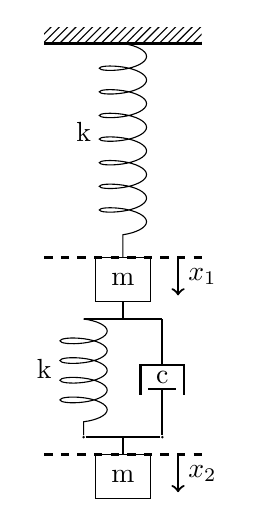
\begin{tikzpicture}
\tikzstyle{damper}=[thick,decoration={markings,  
	mark connection node=dmp,
	mark=at position 0.5 with 
	{
		\node (dmp) [thick,inner sep=0pt,transform shape,rotate=-90,minimum width=15pt,minimum height=8pt,draw=none] {};
		\draw [thick] ($(dmp.north east)+(2pt,0)$) -- (dmp.south east) -- (dmp.south west) -- ($(dmp.north west)+(2pt,0)$);
		\draw [thick] ($(dmp.north)+(0,-5pt)$) -- ($(dmp.north)+(0,5pt)$);
	}
}, decorate]

\node[draw=black,inner sep=2mm] (a) at (0,2) {m};
\draw[dashed,thick] (-1,2.28) -- (1,2.28);
\draw[thick,->] (0.7,2.28) -- (0.7,1.8) node[midway,right] {$x_1$};
\draw[decoration={aspect=0.3, segment length=3mm, amplitude=3mm,coil},decorate] (0,5) -- (a) node[label={[xshift=-0.5cm, yshift=1.5cm]k}] {};
\fill [pattern = north east lines] (-1,5) rectangle (1,5.2);
\draw[thick] (-1,5) -- (1,5);
\draw[thick] (a) -- (0,1.5);
\draw[thick] (-0.5,1.5) -- (0.5,1.5); 
\node[circle,fill=black,inner sep=0pt] (b) at (-0.5,0) {};
\node[circle,fill=black,inner sep=0pt] (c) at (0.5,0) {};
\draw[decoration={aspect=0.3, segment length=2.5mm, amplitude=3mm,coil},decorate] (-0.5,1.5) -- (b) node[label={[xshift=-0.5cm, yshift=0.5cm]k}] {};
\draw [damper] (0.5,1.5) -- (c) node [midway] {c};
\draw[thick] (b)--(c);
\draw[dashed,thick] (-1,-0.22) -- (1,-0.22);
\node[draw=black,inner sep=2mm] (d) at (0,-0.5) {m};
\draw[thick,->] (0.7,-0.22) -- (0.7,-0.7) node[midway,right] {$x_2$};
\draw[thick] (0,0) -- (d);
\end{tikzpicture}
\end{document}